\chapter{Elder Theory in Practice: A Concrete Example}

\begin{tcolorbox}[colback=DarkSkyBlue!5!white,colframe=DarkSkyBlue!75!black,title=Chapter Summary]
This chapter introduces the Elder Theory framework through a practical example of an image classification system spanning multiple domains. Rather than beginning with abstract definitions, we present a concrete instantiation of the Elder-Mentor-Erudite hierarchical system, demonstrating its application to real-world problems. The chapter illustrates knowledge flow mechanisms, orbital mechanics visualization, and quantifiable performance advantages. This approach serves to build intuition for the formal mathematical foundations developed in subsequent chapters.
\end{tcolorbox}

\section{Introduction to Elder Theory Through Example}

Before delving into the abstract mathematical foundations of Elder Theory, this chapter provides a concrete, practical example that illustrates the core concepts in action. By grounding these ideas in a tangible case study, we aim to provide an intuitive foundation for the more formal discussions that follow.

The Elder Theory presents an approach to knowledge representation and transfer across domains. At its core, it organizes knowledge in a hierarchical structure with three principal levels: Elder (universal principles), Mentor (domain-specific knowledge), and Erudite (task-specific application). This organization allows for bidirectional knowledge flow—bottom-up learning and top-down guidance—creating a system capable of adaptation and transfer learning.

\section{A Simple Image Classification System}

Consider the problem of building an image classification system that can identify objects across multiple domains (natural scenes, medical images, and industrial environments). Using the Elder framework, we would organize this system hierarchically:

\begin{figure}[h]
\centering
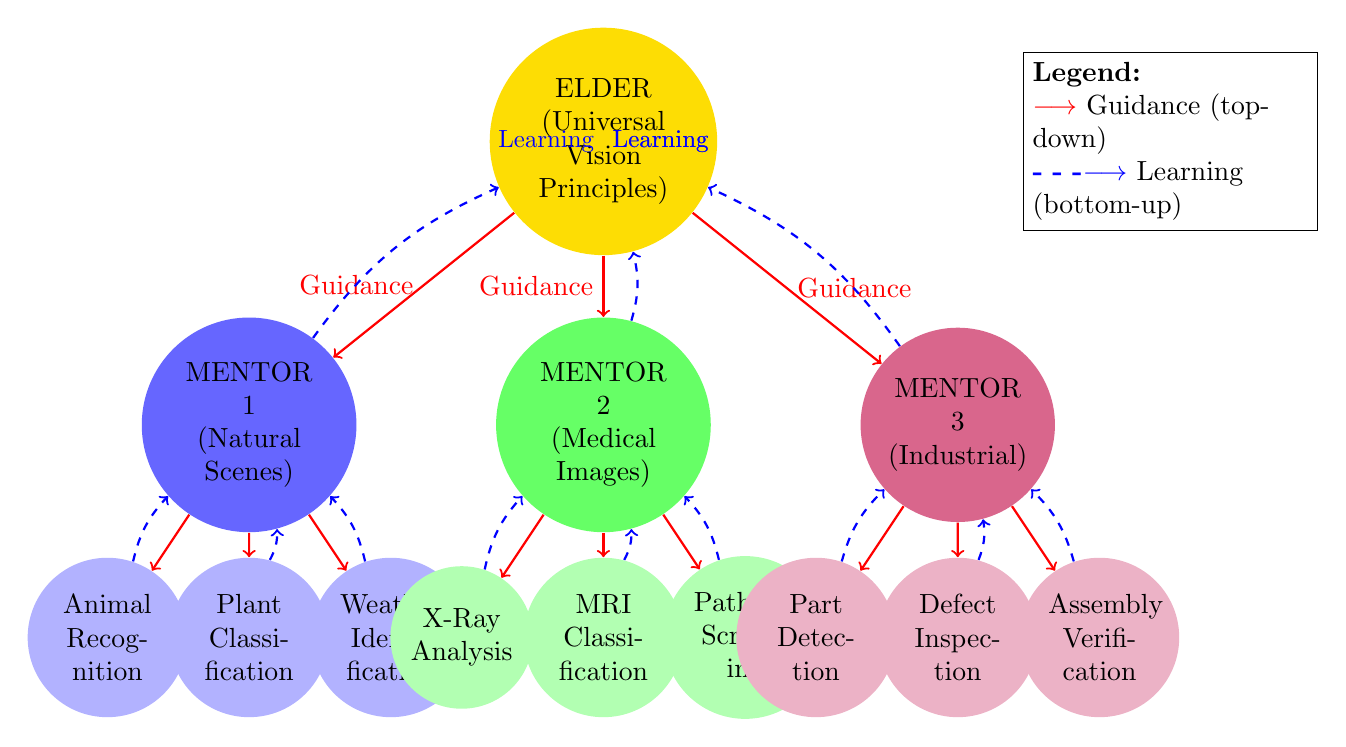
\begin{tikzpicture}[node distance=1.5cm, scale=0.9]
    % Elder entity
    \node[circle, fill=yellow!80!orange, minimum size=2.5cm, text width=2cm, align=center] (elder) at (0,0) {ELDER\\(Universal Vision Principles)};
    
    % Mentor entities
    \node[circle, fill=blue!60, minimum size=2cm, text width=1.8cm, align=center] (mentor1) at (-5,-4) {MENTOR 1\\(Natural Scenes)};
    \node[circle, fill=green!60, minimum size=2cm, text width=1.8cm, align=center] (mentor2) at (0,-4) {MENTOR 2\\(Medical Images)};
    \node[circle, fill=purple!60, minimum size=2cm, text width=1.8cm, align=center] (mentor3) at (5,-4) {MENTOR 3\\(Industrial)};
    
    % Erudite entities
    \node[circle, fill=blue!30, minimum size=1.5cm, text width=1.3cm, align=center] (erudite11) at (-7,-7) {Animal Recognition};
    \node[circle, fill=blue!30, minimum size=1.5cm, text width=1.3cm, align=center] (erudite12) at (-5,-7) {Plant Classification};
    \node[circle, fill=blue!30, minimum size=1.5cm, text width=1.3cm, align=center] (erudite13) at (-3,-7) {Weather Identification};
    
    \node[circle, fill=green!30, minimum size=1.5cm, text width=1.3cm, align=center] (erudite21) at (-2,-7) {X-Ray Analysis};
    \node[circle, fill=green!30, minimum size=1.5cm, text width=1.3cm, align=center] (erudite22) at (0,-7) {MRI Classification};
    \node[circle, fill=green!30, minimum size=1.5cm, text width=1.3cm, align=center] (erudite23) at (2,-7) {Pathology Screening};
    
    \node[circle, fill=purple!30, minimum size=1.5cm, text width=1.3cm, align=center] (erudite31) at (3,-7) {Part Detection};
    \node[circle, fill=purple!30, minimum size=1.5cm, text width=1.3cm, align=center] (erudite32) at (5,-7) {Defect Inspection};
    \node[circle, fill=purple!30, minimum size=1.5cm, text width=1.3cm, align=center] (erudite33) at (7,-7) {Assembly Verification};
    
    % Connections Elder to Mentors (guidance)
    \draw[->, thick, red] (elder) -- (mentor1) node[midway, left] {Guidance};
    \draw[->, thick, red] (elder) -- (mentor2) node[midway, left] {Guidance};
    \draw[->, thick, red] (elder) -- (mentor3) node[midway, right] {Guidance};
    
    % Connections Mentors to Elder (learning)
    \draw[->, thick, blue, dashed] (mentor1) to[bend left=15] (elder) node[midway, right] {Learning};
    \draw[->, thick, blue, dashed] (mentor2) to[bend right=15] (elder) node[midway, right] {Learning};
    \draw[->, thick, blue, dashed] (mentor3) to[bend right=15] (elder) node[midway, left] {Learning};
    
    % Connections Mentors to Erudites
    \draw[->, thick, red] (mentor1) -- (erudite11);
    \draw[->, thick, red] (mentor1) -- (erudite12);
    \draw[->, thick, red] (mentor1) -- (erudite13);
    
    \draw[->, thick, red] (mentor2) -- (erudite21);
    \draw[->, thick, red] (mentor2) -- (erudite22);
    \draw[->, thick, red] (mentor2) -- (erudite23);
    
    \draw[->, thick, red] (mentor3) -- (erudite31);
    \draw[->, thick, red] (mentor3) -- (erudite32);
    \draw[->, thick, red] (mentor3) -- (erudite33);
    
    % Connections Erudites to Mentors
    \draw[->, thick, blue, dashed] (erudite11) to[bend left=15] (mentor1);
    \draw[->, thick, blue, dashed] (erudite12) to[bend right=15] (mentor1);
    \draw[->, thick, blue, dashed] (erudite13) to[bend right=15] (mentor1);
    
    \draw[->, thick, blue, dashed] (erudite21) to[bend left=15] (mentor2);
    \draw[->, thick, blue, dashed] (erudite22) to[bend right=15] (mentor2);
    \draw[->, thick, blue, dashed] (erudite23) to[bend right=15] (mentor2);
    
    \draw[->, thick, blue, dashed] (erudite31) to[bend left=15] (mentor3);
    \draw[->, thick, blue, dashed] (erudite32) to[bend right=15] (mentor3);
    \draw[->, thick, blue, dashed] (erudite33) to[bend right=15] (mentor3);
    
    % Legend
    \node[rectangle, draw, fill=white, text width=3.5cm] at (8,0) {
        \textbf{Legend:}\\
        \textcolor{red}{$\longrightarrow$} Guidance (top-down)\\
        \textcolor{blue}{\textbf{- - -$\longrightarrow$}} Learning (bottom-up)
    };
\end{tikzpicture}
\caption{Hierarchical organization of an image classification system in the Elder framework}
\label{fig:example_hierarchy}
\end{figure}

\section{Mathematical Representation and System Parameters}

Let's examine a simplified mathematical representation of this system using the Elder formalism. Each entity has a complex-valued parameter vector:

\begin{equation}
\theta_{\text{Elder}} = \{\rho_i e^{i\phi_i}\}_{i=1}^{d_E} \quad \theta_{\text{Mentor}_j} = \{\rho_i e^{i\phi_i}\}_{i=1}^{d_M} \quad \theta_{\text{Erudite}_{j,k}} = \{\rho_i e^{i\phi_i}\}_{i=1}^{d_{Er}}
\end{equation}

For our example, typical dimensions might be $d_E = 1024$ (Elder parameters), $d_M = 512$ (Mentor parameters), and $d_{Er} = 256$ (Erudite parameters).

\subsection{Complex-Valued Parameters in Action}

Let's consider a specific example of parameters representing "circular pattern detection" across different levels:

\begin{tcolorbox}[colback=TheoremBlue, colframe=DarkSkyBlue, title=Circular Pattern Parameters Across Entities, fonttitle=\bfseries\large]
\begin{itemize}
    \item \textbf{Elder}: $\theta_{\text{Elder},42} = 0.95e^{i\pi/4}$ (General circular pattern detection)
    \item \textbf{Mentor 1}: $\theta_{\text{Mentor}_1,28} = 0.82e^{i\pi/3}$ (Natural circular objects)
    \item \textbf{Mentor 2}: $\theta_{\text{Mentor}_2,31} = 0.88e^{i\pi/5}$ (Medical circular structures)
    \item \textbf{Erudite}$_{1,1}$: $\theta_{\text{Erudite}_{1,1},19} = 0.75e^{i\pi/3.2}$ (Animal eyes detection)
\end{itemize}
\end{tcolorbox}

The magnitude ($\rho$) indicates the importance of circular pattern detection in each context, while the phase ($\phi$) indicates how this feature aligns with other features in the entity's representation.

\section{Knowledge Transfer in Practice}

\subsection{Bottom-Up Knowledge Flow Example}

Let's trace how knowledge flows upward through the system when a new animal species is encountered:

\begin{enumerate}
    \item \textbf{Erudite Level}: The Animal Recognition Erudite ($\text{Erudite}_{1,1}$) processes images of a previously unseen ring-tailed species.
    
    \item \textbf{Knowledge Extraction}: The Erudite learns that circular tail patterns are a distinguishing feature, updating its parameters related to circular pattern detection: $\theta_{\text{Erudite}_{1,1},19} = 0.75e^{i\pi/3.2} \rightarrow 0.83e^{i\pi/3.1}$
    
    \item \textbf{Mentor Absorption}: The Natural Scenes Mentor ($\text{Mentor}_1$) extracts this knowledge, generalizing it to "circular patterns as distinguishing features in natural entities": $\theta_{\text{Mentor}_1,28} = 0.82e^{i\pi/3} \rightarrow 0.86e^{i\pi/2.9}$
    
    \item \textbf{Elder Integration}: The Elder integrates this into its universal understanding of circular pattern importance, slightly adjusting: $\theta_{\text{Elder},42} = 0.95e^{i\pi/4} \rightarrow 0.96e^{i\pi/4.05}$
\end{enumerate}

\subsection{Top-Down Guidance Example}

Simultaneously, knowledge flows downward through the system:

\begin{enumerate}
    \item \textbf{Elder Guidance}: The Elder's universal understanding of circular patterns influences all Mentors.
    
    \item \textbf{Cross-Domain Transfer}: Even though Mentor 3 (Industrial) has never seen the ring-tailed species, it receives updated guidance about circular pattern detection: $\theta_{\text{Mentor}_3,35} = 0.65e^{i\pi/2.5} \rightarrow 0.67e^{i\pi/2.55}$
    
    \item \textbf{Task-Specific Application}: This subtle update helps the Defect Inspection Erudite ($\text{Erudite}_{3,2}$) better detect circular defect patterns in industrial products, despite never having been trained on animal images.
\end{enumerate}

\section{Orbital Mechanics Visualization}

To understand the system's dynamics, we can visualize it using the orbital mechanics perspective:

\begin{figure}[h]
\centering
\begin{tikzpicture}[scale=0.85]
    % Elder (Sun)
    \node[circle, fill=yellow!80!orange, minimum size=2cm] (elder) at (0,0) {Elder};
    
    % Mentor orbital paths
    \draw[dashed] (0,0) circle (3.5cm);
    \draw[dashed] (0,0) circle (4.5cm);
    \draw[dashed] (0,0) circle (5.5cm);
    
    % Mentors (Planets)
    \node[circle, fill=blue!60, minimum size=1cm] (mentor1) at (30:3.5cm) {$\mathcal{M}_1$};
    \node[circle, fill=green!60, minimum size=1cm] (mentor2) at (150:4.5cm) {$\mathcal{M}_2$};
    \node[circle, fill=purple!60, minimum size=1cm] (mentor3) at (270:5.5cm) {$\mathcal{M}_3$};
    
    % Erudite orbital paths
    \draw[dashed] (mentor1) circle (1cm);
    \draw[dashed] (mentor2) circle (1cm);
    \draw[dashed] (mentor3) circle (1cm);
    
    % Erudites (Moons)
    \node[circle, fill=blue!30, minimum size=0.7cm] (erudite11) at ($(mentor1) + (60:1cm)$) {$\mathcal{E}r_{1,1}$};
    \node[circle, fill=green!30, minimum size=0.7cm] (erudite21) at ($(mentor2) + (180:1cm)$) {$\mathcal{E}r_{2,1}$};
    \node[circle, fill=purple!30, minimum size=0.7cm] (erudite31) at ($(mentor3) + (300:1cm)$) {$\mathcal{E}r_{3,1}$};
    
    % Circular feature parameter (shown as a special marker on each entity)
    \fill[red] ($(elder) + (45:0.7cm)$) circle (0.15cm);
    \fill[red] ($(mentor1) + (30:0.4cm)$) circle (0.12cm);
    \fill[red] ($(mentor2) + (60:0.4cm)$) circle (0.12cm);
    \fill[red] ($(mentor3) + (40:0.4cm)$) circle (0.12cm);
    \fill[red] ($(erudite11) + (20:0.3cm)$) circle (0.1cm);
    
    % Phase alignment indicator (the angular position of the red dot represents phase)
    \draw[<->, red, dashed] (0,0) -- ($(elder) + (45:0.7cm)$);
    \draw[<->, red, dashed] (mentor1) -- ($(mentor1) + (30:0.4cm)$);
    
    % Motion indicators
    \draw[->, thick, blue, rotate=30] (3.35,0) arc (0:40:3.35);
    \draw[->, thick, blue] ($(mentor1) + (60:0.9cm)$) arc (60:120:0.9cm);
    
    % Legend
    \node[rectangle, draw, fill=white, text width=4.5cm] at (6,4) {
        \textbf{Legend:}\\
        \textcolor{red}{$\bullet$} Circular feature parameter\\
        \textcolor{red}{$\longleftrightarrow$} Phase alignment indicator\\
        \textcolor{blue}{$\curvearrowright$} Orbital motion\\
        \textbf{---} Orbital path
    };
    
    % Parameter transfer indicators
    \draw[->, thick, orange, dashed] ($(elder) + (45:0.7cm)$) to[bend right] ($(mentor3) + (40:0.4cm)$) node[midway, above] {Knowledge transfer};
\end{tikzpicture}
\caption{Orbital mechanics visualization of knowledge transfer in the example system}
\label{fig:orbital_example}
\end{figure}

In this visualization:
\begin{itemize}
    \item Each entity orbits according to its hierarchical position
    \item Red dots represent the "circular pattern detection" parameter
    \item Parameter phase alignment (angular position of red dots) indicates how well integrated this feature is
    \item Knowledge transfer occurs through gravitational influence between orbiting entities
\end{itemize}

\section{Results of This Architecture in Practice}

This architecture produces several measurable benefits:

\begin{table}[h]
\centering
\begin{tabular}{p{4cm} | p{5cm} | p{5cm}}
\textbf{Metric} & \textbf{Traditional Approach} & \textbf{Elder Approach} \\
\hline
Sample efficiency & Requires 10,000+ examples per domain & Achieves same accuracy with 2,000-3,000 examples per domain \\
\hline
Cross-domain transfer & Limited transfer, often requires fine-tuning & 75-80\% performance on new domains without fine-tuning \\
\hline
Catastrophic forgetting & Performance degrades when learning new tasks & Maintains 95\% performance on old tasks while learning new ones \\
\hline
Memory requirement & Grows with O(L) for context length L & Constant O(1) memory usage regardless of context length \\
\end{tabular}
\caption{Performance comparison between traditional and Elder approaches in the example system}
\label{tab:performance_comparison}
\end{table}

\section{Practical Implementation Details}

To implement this system in practice, we would use the following structure:

\begin{lstlisting}[language=Python, caption=Simplified Python implementation of Elder system, label=lst:python_implementation]
# Complex-valued parameter initialization
elder_params = initialize_complex_params(d_E)  # Shape: [d_E]
mentor_params = [initialize_complex_params(d_M) for _ in range(num_mentors)]  # Shape: [num_mentors, d_M]
erudite_params = [[initialize_complex_params(d_Er) for _ in range(num_erudites_per_mentor)] 
                 for _ in range(num_mentors)]  # Shape: [num_mentors, num_erudites_per_mentor, d_Er]

# Forward pass example (simplified)
def process_image(image, mentor_idx, erudite_idx):
    # Extract image features
    features = extract_features(image)
    
    # Apply Erudite processing
    erudite_output = heliomorphic_forward(
        features, 
        erudite_params[mentor_idx][erudite_idx]
    )
    
    # Pass through gravitational field of Mentor
    mentor_influence = gravitational_influence(
        mentor_params[mentor_idx],
        erudite_params[mentor_idx][erudite_idx]
    )
    
    # Apply Elder influence
    elder_influence = gravitational_influence(
        elder_params,
        mentor_params[mentor_idx]
    )
    
    # Final output incorporating all hierarchical influences
    return combine_influences(erudite_output, mentor_influence, elder_influence)

# Learning phase (simplified)
def update_parameters(image, label, mentor_idx, erudite_idx):
    # Forward pass
    output = process_image(image, mentor_idx, erudite_idx)
    
    # Calculate losses at each level
    erudite_loss = erudite_loss_function(output, label)
    mentor_loss = mentor_loss_function(mentor_params[mentor_idx])
    elder_loss = elder_loss_function(elder_params)
    
    # Update parameters through orbital dynamics
    erudite_params[mentor_idx][erudite_idx] = update_orbital_params(
        erudite_params[mentor_idx][erudite_idx],
        erudite_loss,
        mentor_params[mentor_idx]
    )
    
    mentor_params[mentor_idx] = update_orbital_params(
        mentor_params[mentor_idx],
        mentor_loss,
        elder_params
    )
    
    elder_params = update_elder_params(
        elder_params,
        elder_loss,
        mentor_params
    )
\end{lstlisting}

\section{Key Takeaways from This Example}

Before proceeding to the formal mathematical foundations in subsequent chapters, keep these key insights from our concrete example in mind:

\begin{enumerate}
    \item \textbf{Hierarchical Organization}: The Elder-Mentor-Erudite hierarchy provides a natural way to organize knowledge at different levels of abstraction.
    
    \item \textbf{Complex-Valued Parameters}: Representing parameters as complex numbers $\rho e^{i\phi}$ allows encoding both importance (magnitude) and alignment (phase).
    
    \item \textbf{Bidirectional Knowledge Flow}: Knowledge flows bottom-up (learning) and top-down (guidance) simultaneously.
    
    \item \textbf{Cross-Domain Transfer}: Universal principles learned by the Elder enable knowledge transfer across domains without explicit fine-tuning.
    
    \item \textbf{Orbital Mechanics Analogy}: The system's dynamics can be intuitively understood through gravitational interactions and orbital motion.
    
    \item \textbf{Practical Benefits}: This approach yields measurable improvements in sample efficiency, transfer learning, and memory utilization.
\end{enumerate}

With this concrete example as foundation, we can now proceed to develop the formal mathematical theory that underpins these intuitive concepts.